\section{Resultados e discussão}
\label{sec:resultados}

\subsection{Estrutura bibliométrica e evolução do campo}
\label{sec:panorama}

O núcleo temático vigente reúne 121 registros publicados entre 2010 e 2026, dos quais 104 pertencem ao núcleo original e 17 foram incorporados pela busca de sensibilidade para inteligência artificial e aprendizado de máquina (Seção~\ref{sec:buscaia}). Entre 2019 e 2026 concentram-se 101 registros (83,5\%), com máximo de 29 estudos em 2025 (Gráfico~\ref{fig:temporal}). A deduplicação preservou a proveniência múltipla. Sessenta e sete registros vieram apenas da Scopus, 41 da Scopus e da Web of Science, sete apenas da Web of Science, três das três bases, dois da Scopus e do Crossref e um apenas do Crossref (Tabela~\ref{tab:basetipo}). A baixa disponibilidade de resumos no Crossref reduziu sua contribuição à triagem.

\begin{figure}[htbp]
\centering
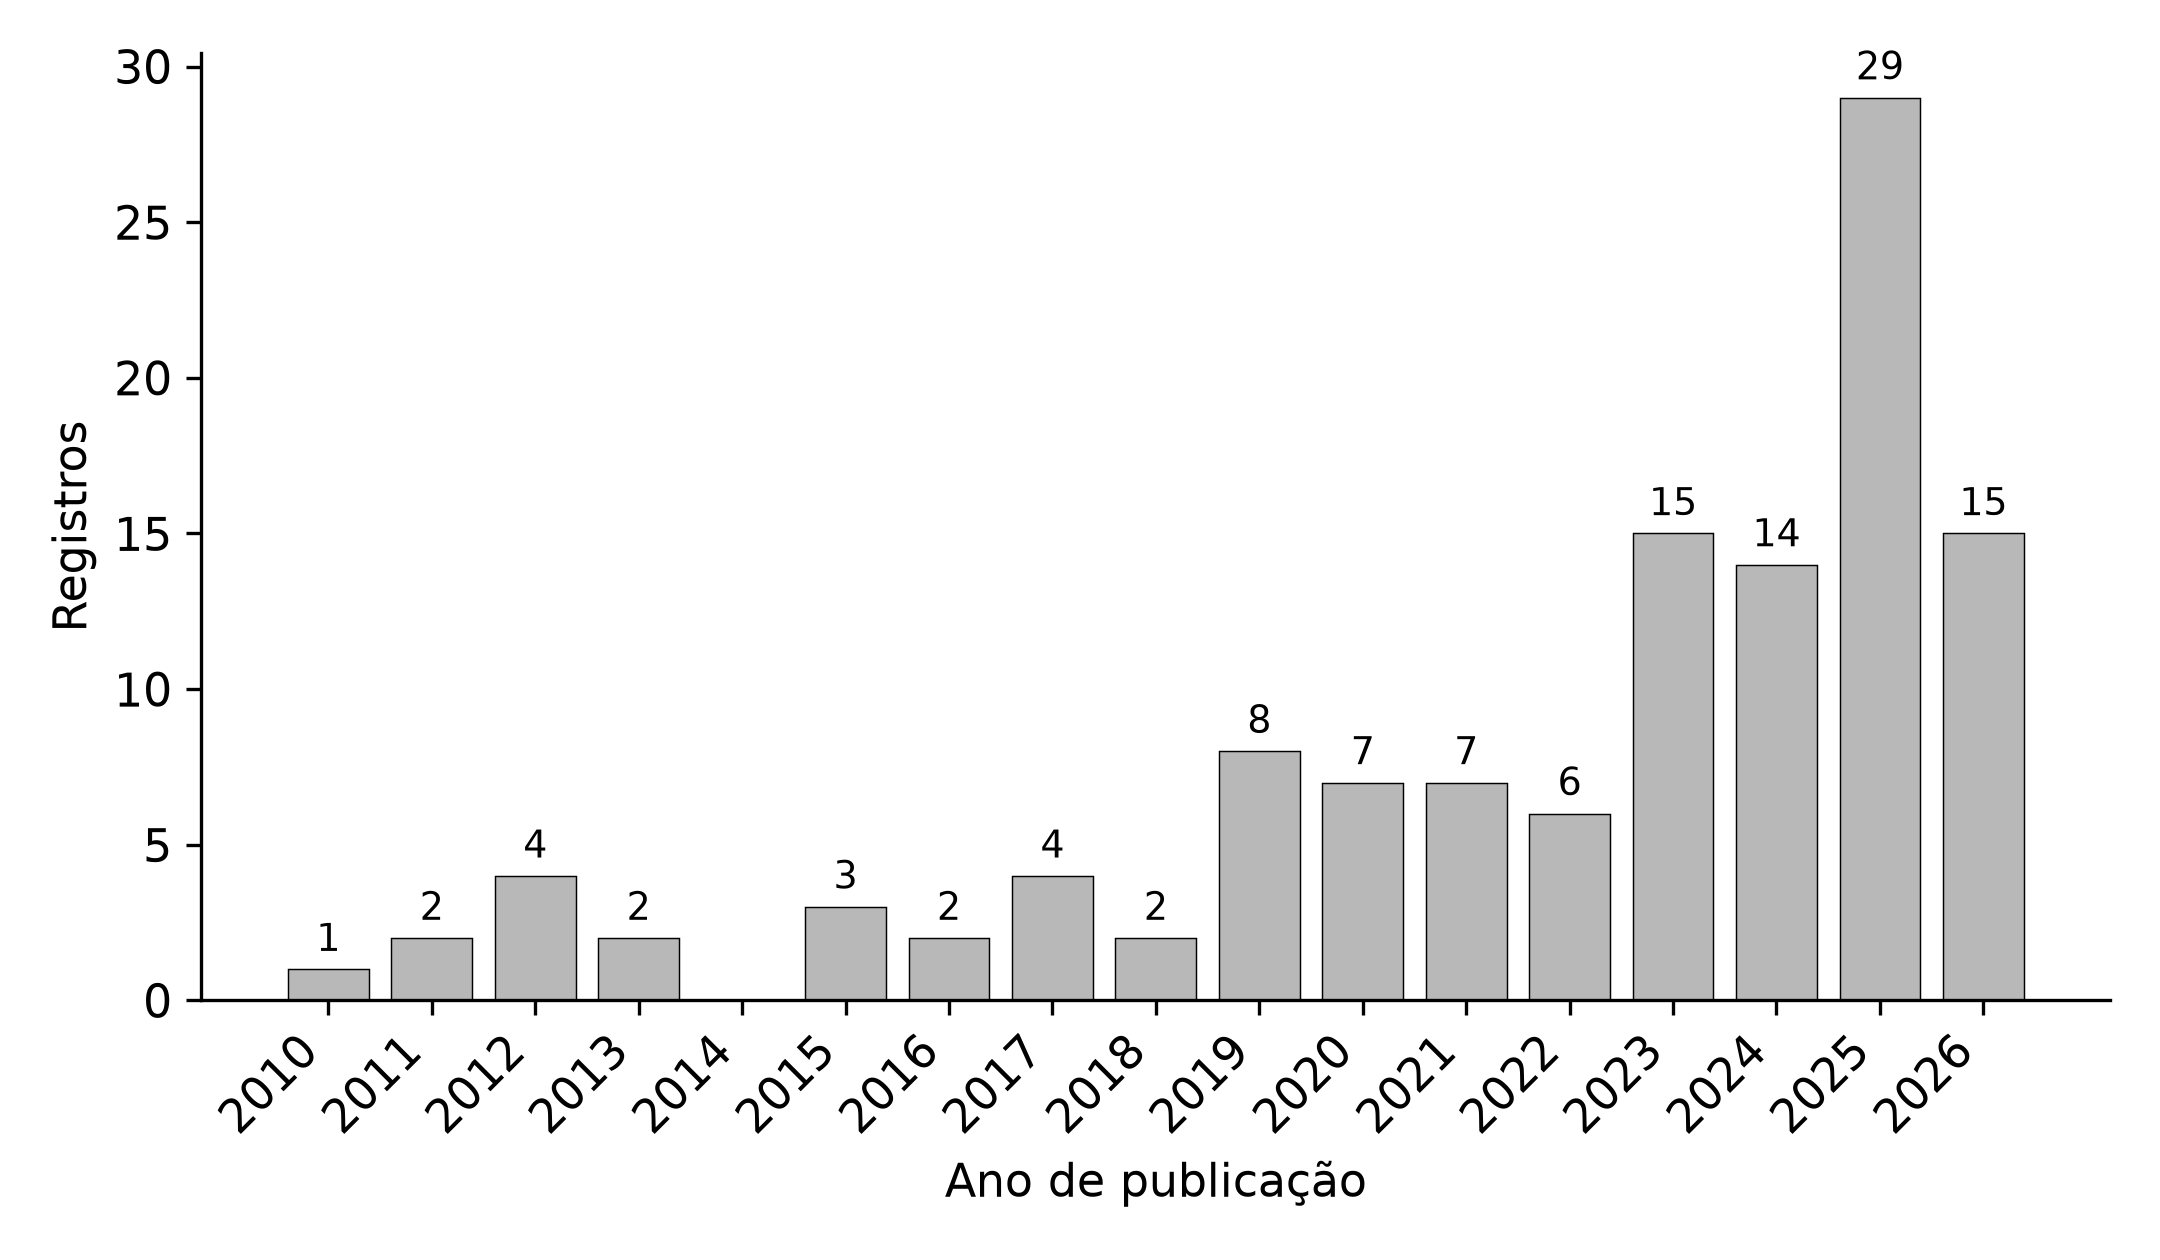
\includegraphics[width=0.9\linewidth]{figuras/figura09_distribuicao_temporal_nucleo_ampliado_121.png}
\captiongrafico{Distribuição temporal do núcleo temático vigente}
\label{fig:temporal}
\end{figure}

Os tipos documentais foram harmonizados, reunindo \textit{Journal}, \textit{JOUR} e \textit{journal-article} na categoria artigo de periódico; \textit{Conference Proceeding} e \textit{CPAPER} em trabalhos em evento; \textit{Book Series} e \textit{Book} em livro ou série de livro. A Tabela~\ref{tab:basetipo} apresenta proveniência e tipologia separadamente, indicando predomínio de artigos de periódico e forte presença da Scopus; a sobreposição entre bases registra caminhos de recuperação do mesmo estudo, enquanto a avaliação da evidência depende do conteúdo de cada registro.

\begin{table}[htbp]
\centering
\caption{Distribuição do núcleo temático vigente por base de origem e tipo documental}
\label{tab:basetipo}
\footnotesize
\begin{tabularx}{\textwidth}{>{\RaggedRight\arraybackslash}p{3.7cm} >{\raggedleft\arraybackslash}p{1.8cm} >{\raggedleft\arraybackslash}p{1.8cm} Y}
\toprule
Categoria & Registros & \% dos 121 & Observação \\
\midrule
\multicolumn{4}{l}{\textbf{A. Registros do núcleo com origem na base, respostas múltiplas}} \\
Scopus & 113 & 93,4 & Base bibliográfica principal. \\
Web of Science & 51 & 42,1 & Base bibliográfica independente. \\
Crossref & 6 & 5,0 & Fonte complementar de metadados. \\
\addlinespace
\multicolumn{4}{l}{\textbf{B. Tipo documental harmonizado, categorias exclusivas}} \\
Artigo de periódico & 90 & 74,4 & \textit{Journal}, \textit{JOUR} e \textit{journal-article}. \\
Trabalho em evento & 20 & 16,5 & \textit{Conference Proceeding} e \textit{CPAPER}. \\
Livro ou série de livro & 11 & 9,1 & \textit{Book Series} e \textit{Book}. \\
\bottomrule
\end{tabularx}
\fonteautor
\end{table}

A camada bibliométrica, com função analítica distinta da síntese temática (cf. Método), utilizou os 372 registros com aderência simultânea ao objeto predial, à manutenção ou gestão, à sustentabilidade e à presença de método, dados ou resultados; 329 (88,4\%) continham palavras-chave, 327 (87,9\%) DOI e 91 (24,5\%) autores. As palavras-chave foram normalizadas quanto a caixa, acentuação, singular e variantes ortográficas, reunindo, por exemplo, \textit{building information modeling}, \textit{building information modelling} e BIM; a rede considera a coocorrência no mesmo registro, normalizada pelo cosseno das frequências marginais, e a evolução compara 157 registros de 2010--2020 com 215 de 2021--2026.

O Gráfico~\ref{fig:fontes372} sintetiza 208 fontes, das quais o núcleo aproximado de Bradford reuniu 13, responsáveis por cerca de um terço dos registros, entre elas \textit{Energy and Buildings} (18), \textit{Journal of Building Engineering} (15), \textit{Facilities} (14), \textit{Lecture Notes in Civil Engineering} (11), \textit{IOP Conference Series: Earth and Environmental Science} (10) e \textit{Sustainability} (10), confirmando a interdisciplinaridade entre energia, engenharia de edificações, gestão de facilidades e sustentabilidade.

\begin{figure}[htbp]
\centering
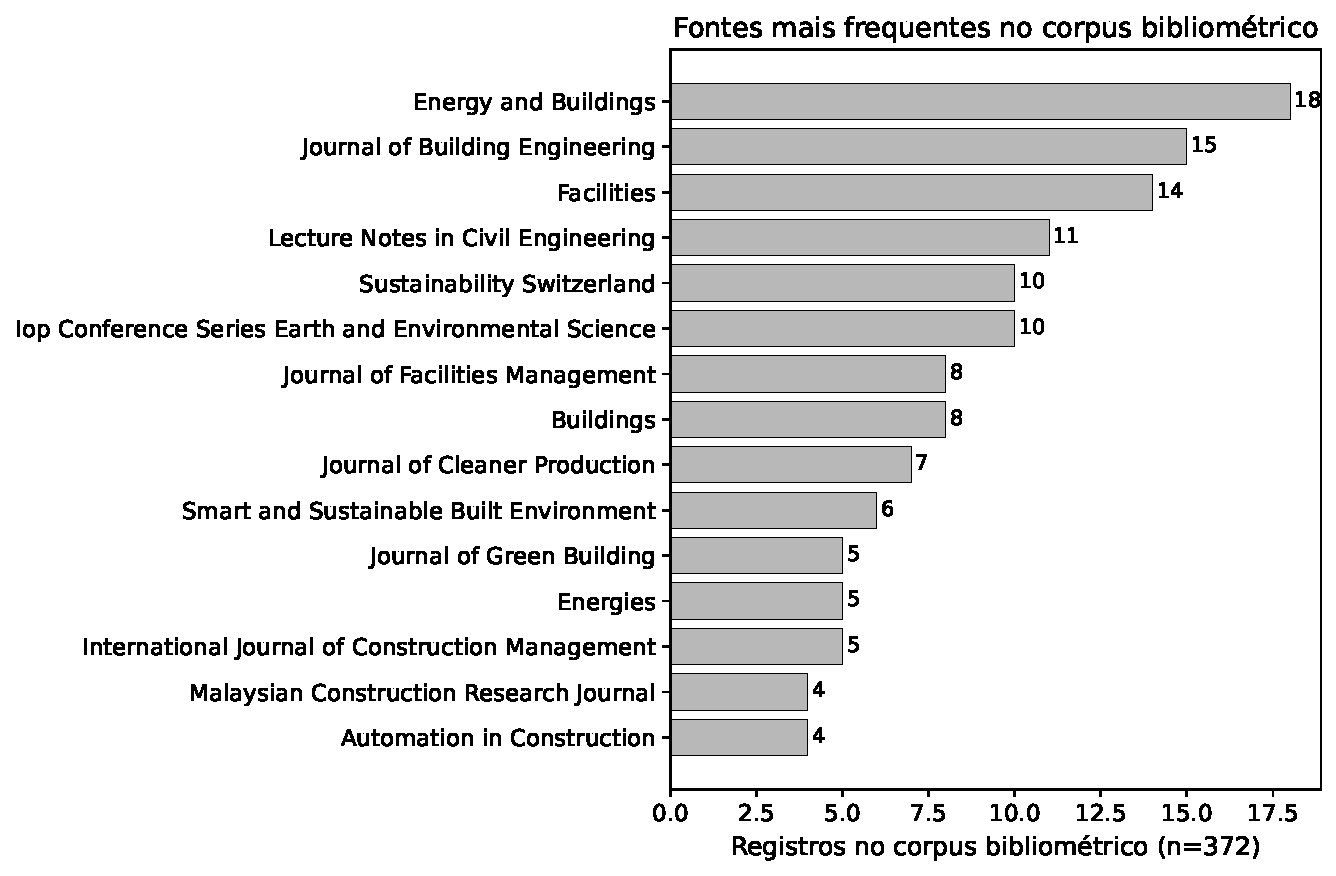
\includegraphics[width=0.98\linewidth]{figuras/figura_fontes_relevantes_372.pdf}
\captiongrafico{Fontes mais frequentes no corpus bibliométrico ampliado}
\label{fig:fontes372}
\end{figure}

O mapa temático (Gráfico~\ref{fig:mapatematico372}) revelou dois eixos centrais, formados por BIM, desempenho da edificação e \textit{digital twins}, com centralidade e densidade acima das medianas, e gestão de facilidades, edifícios inteligentes e manutenção preditiva, com elevada centralidade e menor densidade interna. Edificações verdes, avaliação do ciclo de vida e desenvolvimento sustentável formaram grupos mais especializados, enquanto energia, emissões e operação predial permaneceram semanticamente heterogêneas.

\begin{figure}[htbp]
\centering
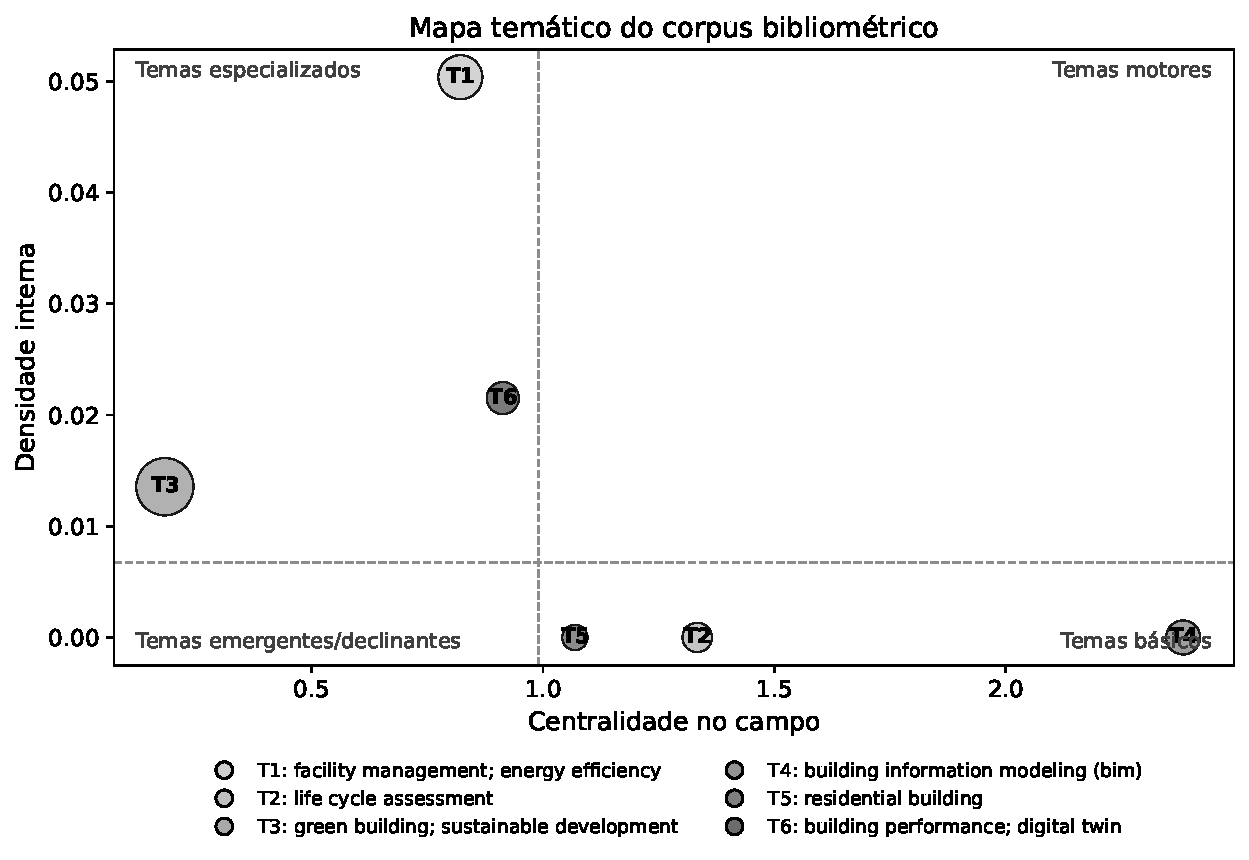
\includegraphics[width=0.98\linewidth]{figuras/figura_mapa_tematico_372.pdf}
\captiongrafico{Mapa temático por centralidade e densidade das palavras-chave}
\label{fig:mapatematico372}
\end{figure}

A rede normalizada (Gráfico~\ref{fig:redecor372}) reforça BIM e gestão de facilidades como conectores centrais, associados a \textit{digital twins}, manutenção preditiva, operação, desempenho, gestão de ativos e internet das coisas; em outro agrupamento, avaliação do ciclo de vida aproxima-se de edificações residenciais e desenvolvimento sustentável.

\begin{figure}[htbp]
\centering
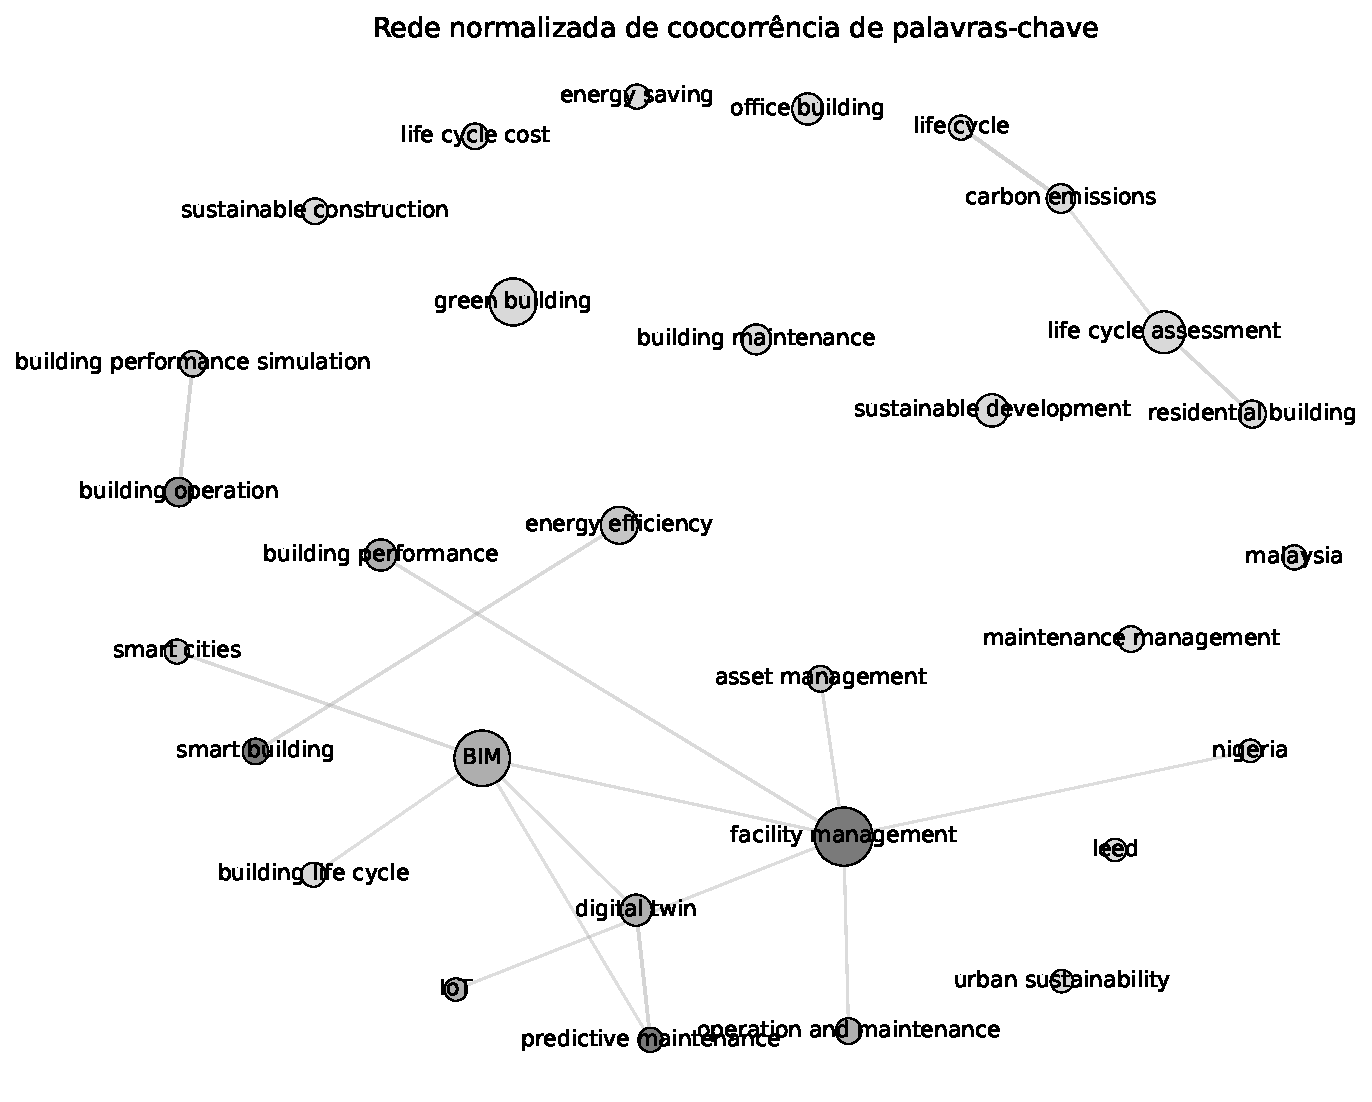
\includegraphics[width=0.98\linewidth]{figuras/figura_rede_coocorrencia_372.pdf}
\captiongrafico{Rede normalizada de coocorrência de palavras-chave}
\label{fig:redecor372}
\end{figure}

A comparação temporal (Gráfico~\ref{fig:evolucaotematica372}) mostrou aumento de 7,3 pontos percentuais para BIM, 4,7 para \textit{digital twins}, 2,7 para emissões de carbono e 1,9 para avaliação do ciclo de vida, enquanto edificação verde, eficiência energética, manutenção predial e desempenho da edificação perderam participação relativa. Esse movimento descreve uma associação documental de transição lexical, compatível com a incorporação de temas tradicionais a vocabulários tecnológicos e de ciclo de vida mais específicos, sem implicar relação causal entre os termos.

\begin{figure}[htbp]
\centering
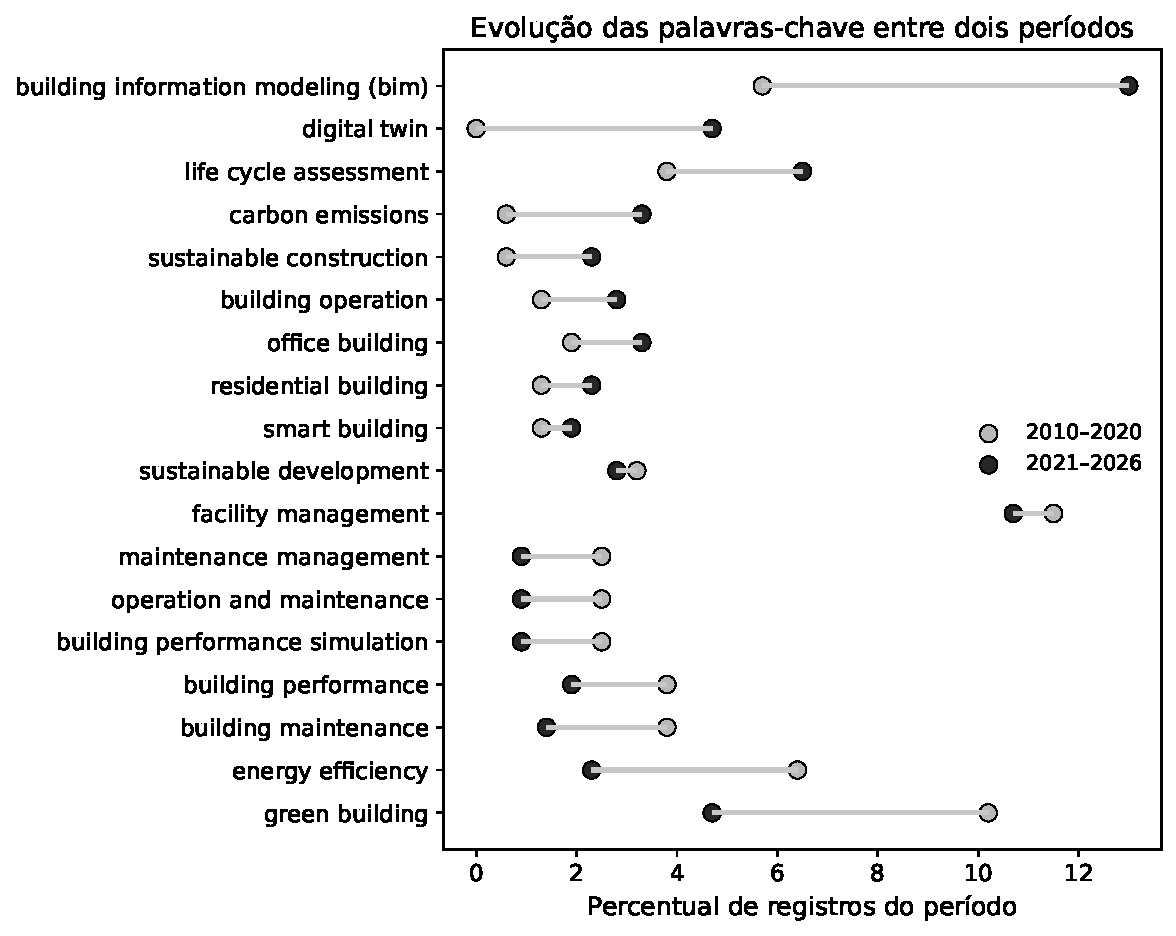
\includegraphics[width=0.98\linewidth]{figuras/figura_evolucao_tematica_372.pdf}
\captiongrafico{Evolução das palavras-chave entre 2010--2020 e 2021--2026}
\label{fig:evolucaotematica372}
\end{figure}

Em conjunto, a bibliometria indica transição de eficiência, desempenho e edificações verdes para BIM, \textit{digital twins}, carbono, ciclo de vida e manutenção preditiva, embora o crescimento informacional não implique, por si, integração decisória equivalente. As subseções seguintes verificam como essa transição se converte em dimensões, critérios, métodos e regras aplicáveis à priorização pública universitária.

\subsection{Dimensões e critérios para priorização sustentável}
\label{sec:criterios}

Foram identificadas seis dimensões com respostas múltiplas, na ordem técnica-operacional (116 registros), institucional (97), ambiental (92), ciclo de vida (65), econômica (63) e social (59). O predomínio das duas primeiras reflete a amplitude do manual de codificação e descreve a composição documental do núcleo, convergindo com a gestão sustentável de facilidades, que articula impactos ambientais, sociais e econômicos nos níveis estratégico, tático e operacional \parencite{nielsen_sustentabilidadefm_2016,okoro_sustainablefm_2023}, e com avaliações educacionais que integram desempenho, energia, conforto e usuários \parencite{alfalah_frameworkeducacional_2022}.

\begin{figure}[htbp]
\centering
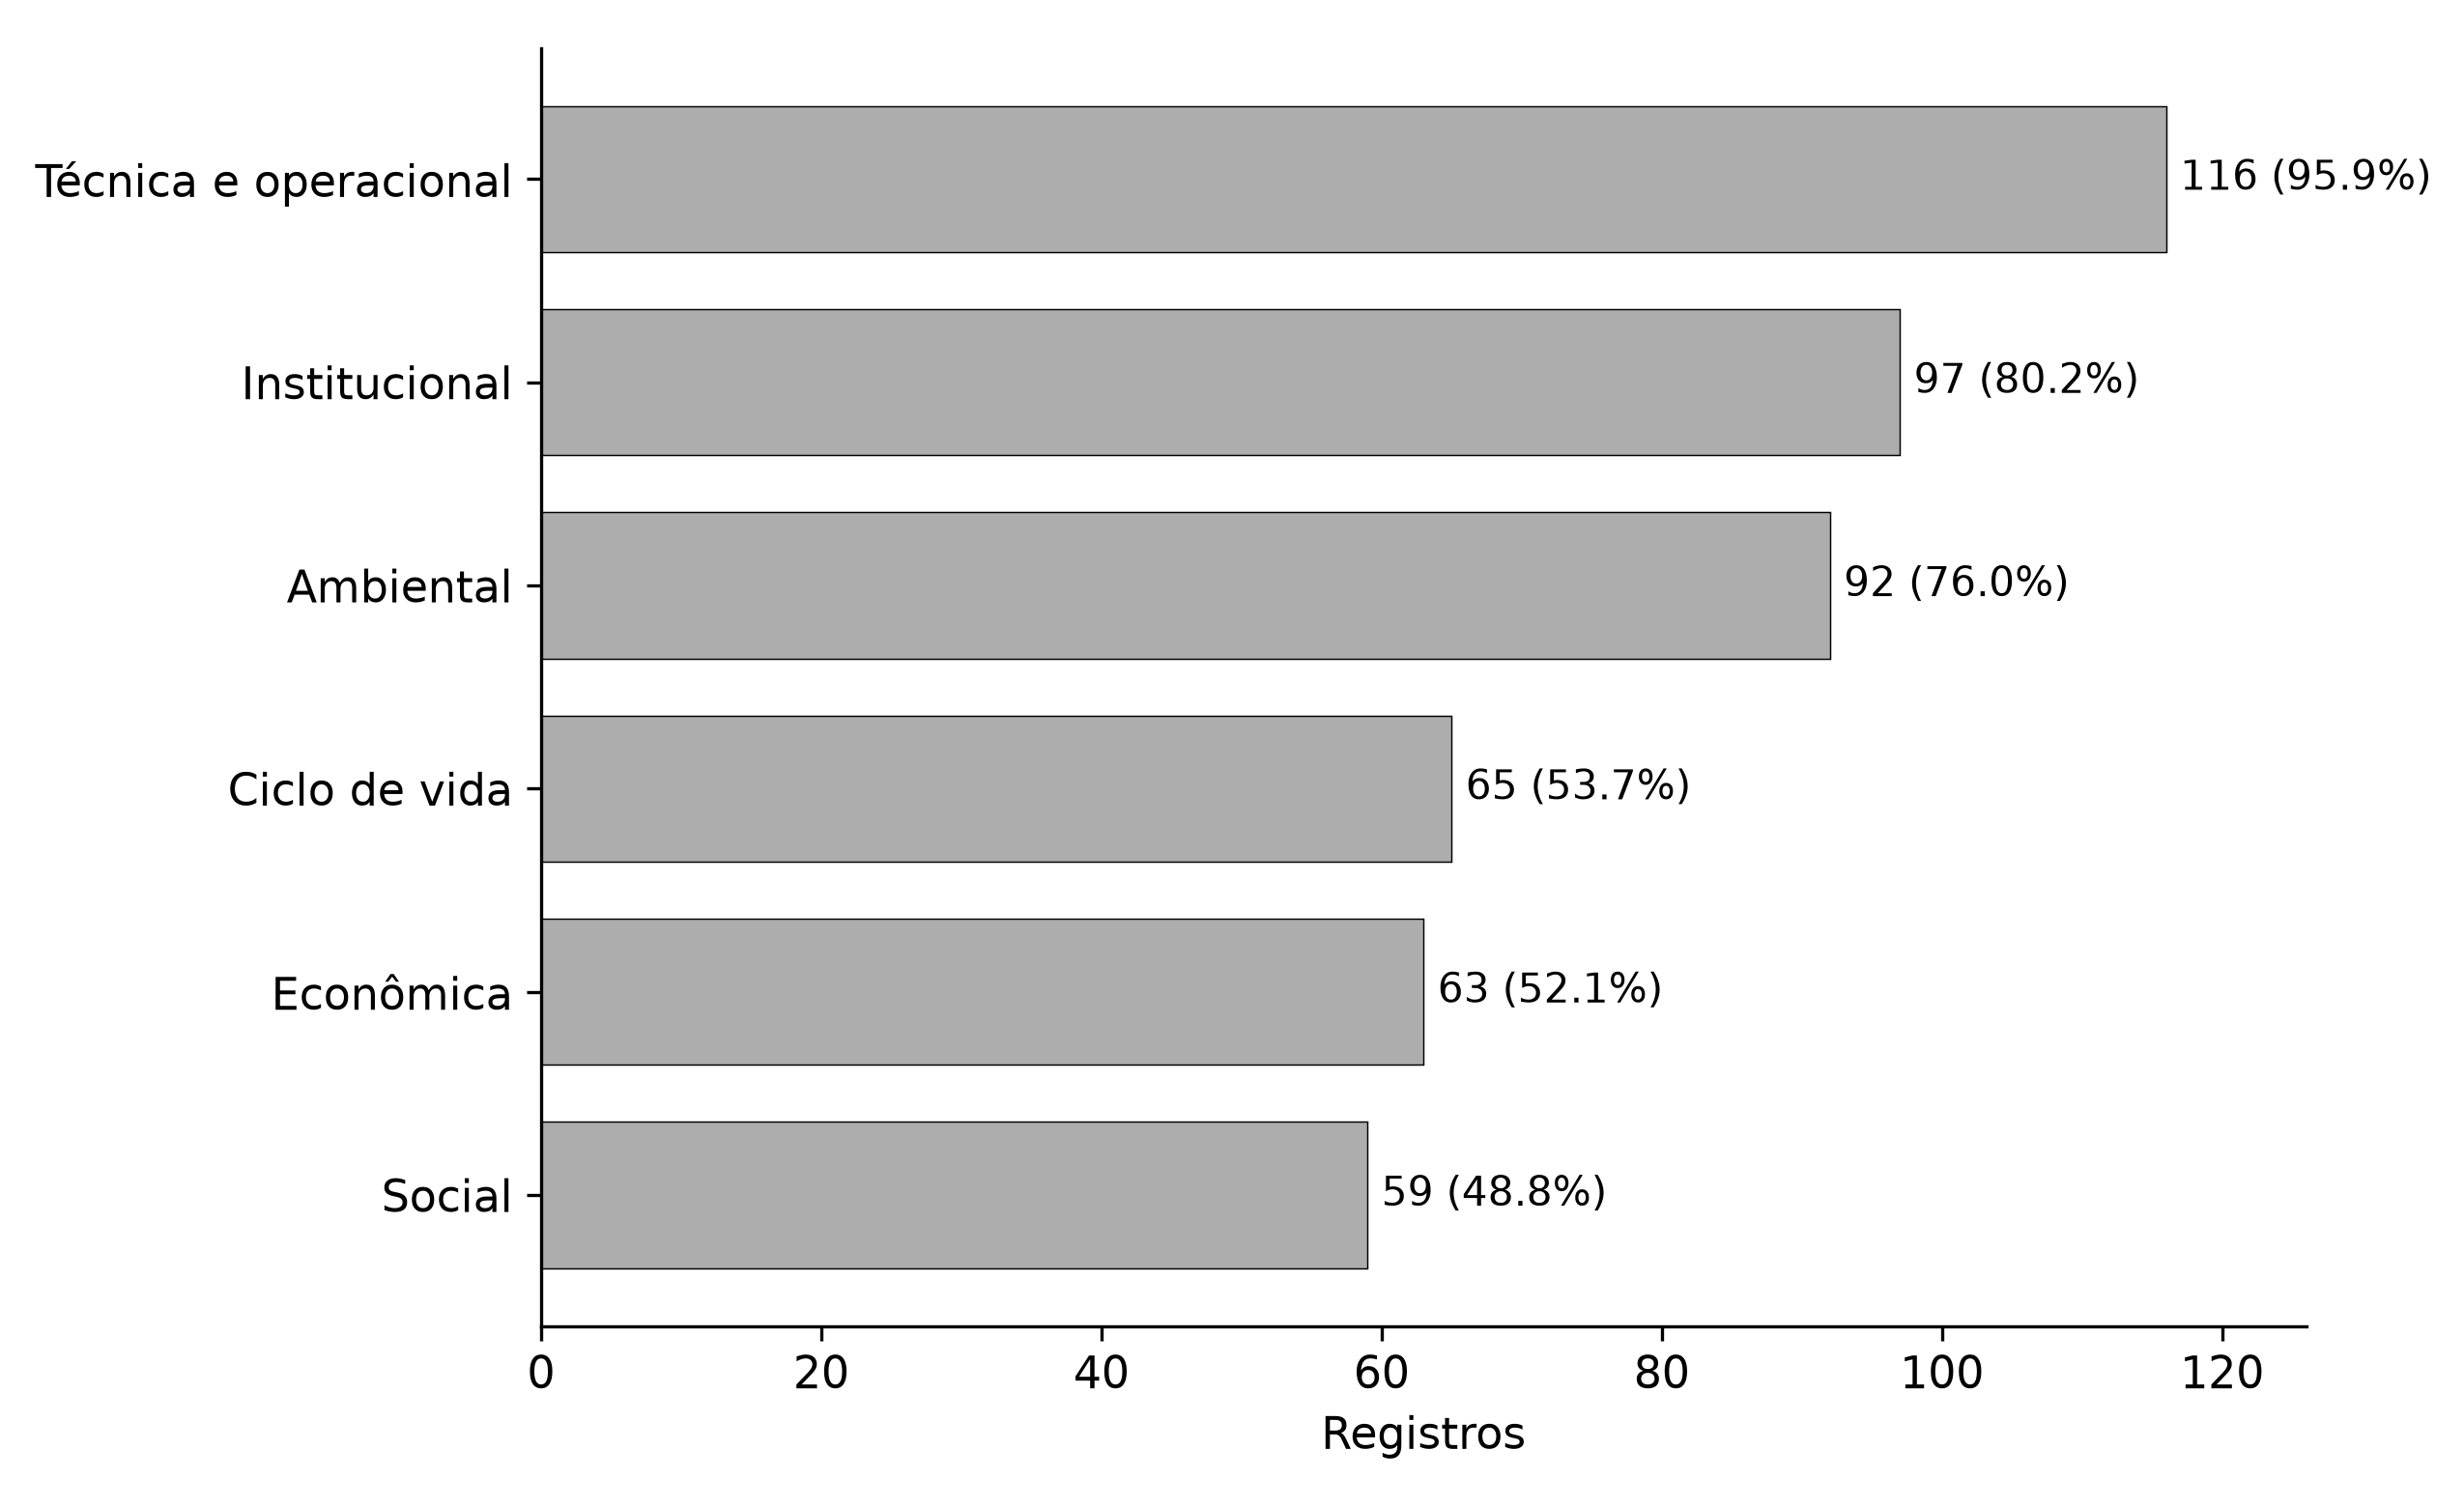
\includegraphics[width=0.90\linewidth]{figuras/figura12_dimensoes_sustentabilidade_nucleo_ampliado_121.png}
\captiongrafico{Dimensões de sustentabilidade identificadas no núcleo temático vigente}
\label{fig:dimensoes}
\end{figure}

Os ODS apareceram explicitamente em um registro, que combinou sustentabilidade, AHP, TOPSIS e otimização na alocação de prestadores de manutenção pública \parencite{masmoudi_ahptopsis_2026}; o vocabulário ESG esteve ausente dos campos auditados, embora componentes ambientais, sociais e institucionais fossem frequentes, padrão compatível com sua incorporação ainda emergente à gestão de facilidades \parencite{ramantswana_esgfm_2026}.

Quanto aos critérios de priorização, desempenho operacional apareceu em 99 registros, informação e dados em 82, custo em 63 e energia e vida útil em 44 cada, com os demais critérios técnicos, sociais e ambientais listados na Tabela~\ref{tab:criteriospriorizacao}.

\begin{table}[htbp]
\centering
\caption{Critérios de priorização identificados no núcleo temático vigente}
\label{tab:criteriospriorizacao}
\small
\begin{tabularx}{\textwidth}{Y >{\raggedleft\arraybackslash}p{2.1cm} >{\raggedleft\arraybackslash}p{2.1cm}}
\toprule
Critério & Registros & \% dos 121 \\
\midrule
Desempenho operacional & 99 & 81,8 \\
Informação e dados & 82 & 67,8 \\
Custo & 63 & 52,1 \\
Energia & 44 & 36,4 \\
Vida útil & 44 & 36,4 \\
Condição física & 34 & 28,1 \\
Risco & 33 & 27,3 \\
Manutenibilidade & 25 & 20,7 \\
Conforto & 22 & 18,2 \\
Segurança & 18 & 14,9 \\
Emissões de carbono & 15 & 12,4 \\
Resíduos & 13 & 10,7 \\
Satisfação do usuário & 9 & 7,4 \\
Água & 6 & 5,0 \\
Qualidade de serviço & 6 & 5,0 \\
\bottomrule
\end{tabularx}
\fonteautor
\end{table}

Na gestão pública universitária, o desempenho sustenta indicadores relacionados à continuidade e às falhas, a informação oferece as condições necessárias à rastreabilidade e o custo permite distinguir correções emergenciais, manutenção planejada e renovação, combinação reforçada por registros de pagamento e planejamento conjunto de manutenção, renovação e energia \parencite{kim_estimativacustoseducacional_2018,nageli_ciclovida_2019}. As leituras integrais qualificam relações entre critérios. Operação e manutenção podem superar 80\% do custo total do ciclo de vida, e seus custos anuais podem representar de 50\% a 70\% dos custos operacionais, bases de cálculo que devem permanecer distintas \parencite{aliu_barreirasdt_2025}; decisões de concepção podem evitar até 50\% das dificuldades de manutenção, conectando manutenibilidade a desempenho, custo e risco \parencite{othman_manutenibilidadeesi_2023,chew_manutenibilidadeverde_2016,conejos_verticalgreenery_2019}.

\subsection{Digitalização, IA e métodos de apoio à decisão}
\label{sec:metodos}

Sobre os métodos de apoio à decisão, a categoria ampla \texttt{framework} reuniu 101 registros. BIM apareceu em 28 e a categoria \texttt{decision\_support}, definida no manual como presença de mecanismo explícito de apoio à decisão, em 29; seguiram-se aprendizado de máquina em 26, otimização em 19, pontuação em 17 e custo do ciclo de vida em 16. Entre os métodos nomeados, AHP ocorreu em cinco registros, TOPSIS em quatro, MCDM e Delphi em três cada, ANP em dois, e \textit{Bayesian Best-Worst Method}, \textit{balanced scorecard} e raciocínio baseado em casos em um cada. Essa predominância de estruturas genéricas sobre métodos multicritério nomeados marca a transição do campo, cujo avanço informacional é mais rápido que a integração decisória.

\begin{figure}[htbp]
\centering
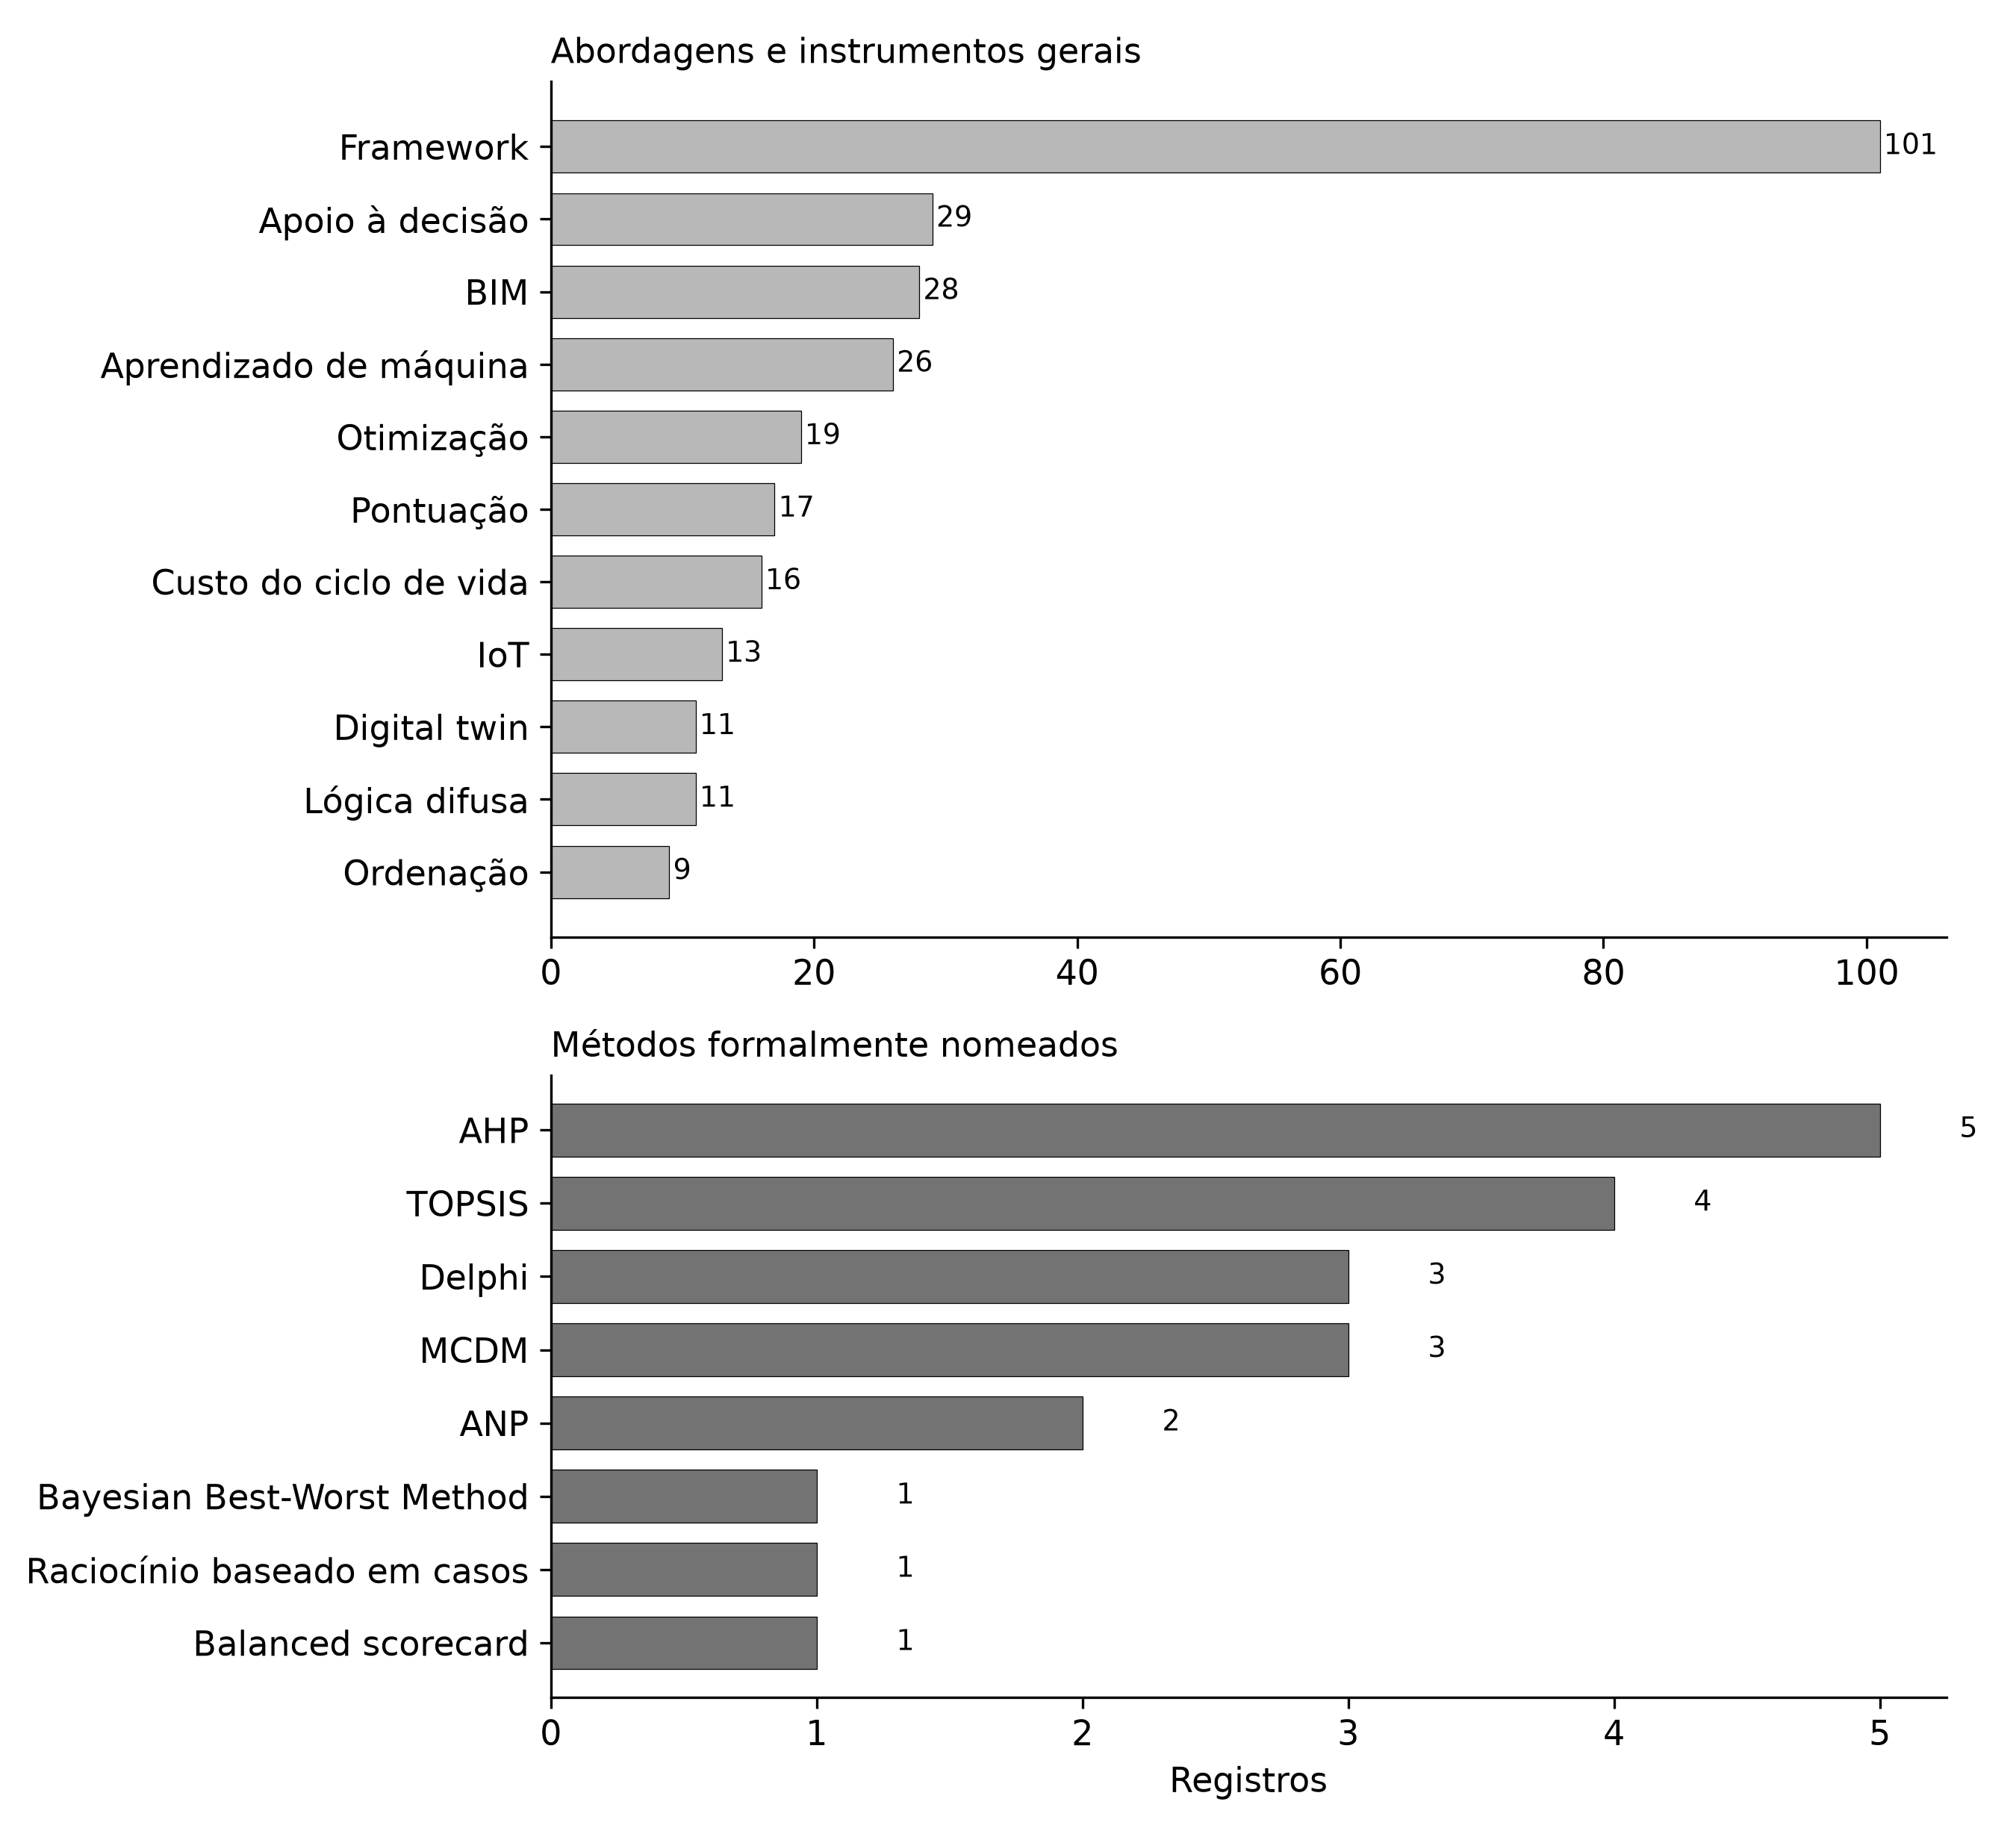
\includegraphics[width=0.95\linewidth]{figuras/figura11_metodos_mcdm_mais_frequentes_nucleo_ampliado_121.png}
\captiongrafico{Abordagens e métodos de apoio à decisão identificados no núcleo temático vigente}
\label{fig:metodos}
\end{figure}

\textit{Digital twin} foi identificado em 11 registros (9,1\%), e a busca de sensibilidade elevou o aprendizado de máquina de nove para 26 registros (21,5\%), resultado diretamente associado ao enriquecimento temático da rodada complementar. Para a especificação proposta, a arquitetura informacional pode começar com planilhas, cadastros, inspeções e ordens de serviço e evoluir para plataformas digitais e módulos preditivos conforme a qualidade dos dados. As aplicações multicritério identificadas desempenham funções distintas, como o ANP difuso na avaliação de edifícios educacionais \parencite{alfalah_frameworkeducacional_2022}, Delphi modificado na gestão de \textit{campus} \parencite{naji_campusdelphi_2023} e a combinação de AHP, TOPSIS e otimização na alocação de prestadores públicos \parencite{masmoudi_ahptopsis_2026}.

A leitura integral do lote da RQ6 separa produção de variáveis operacionais e governança decisória. Modelos de aprendizado de máquina estimaram demanda de ventilação, com economia de até 7,5\% sobre o controle tradicional \parencite{motuziene_ventilacaoia_2025}, vida útil de componentes por regressão em grafos, com $R^2=0{,}83$ \parencite{wu_gnnvidautil_2025}, e consumo de eletricidade, gás e água com conjuntos separados de treinamento, validação e teste \parencite{suh_demandaenergiaagua_2012}, além de diagnóstico, classificação de danos e apoio operacional. Duas revisões qualificam esse alcance. A síntese de IoT e IA identificou concentração no Norte Global e desafios de interoperabilidade, privacidade, governança e ciclo de vida \parencite{das_iotai_2025}, e entre 76 estudos sobre ambientes internos conectados, 41 integraram energia, conforto e sustentabilidade e 35 apenas parte delas \parencite{alici_iotambientes_2026}. A matriz comparativa dos 17 registros, no material suplementar, classifica dez estudos em previsão ou previsão com otimização, dois em diagnóstico e classificação de danos e cinco em síntese ou integração tecnológica, e apenas três aproximam a saída de uma ação operacional. A integração com preferências institucionais, ponderação e vetos permanece etapa decisória adicional.

As leituras do núcleo original ampliam essa distinção. A revisão de 123 estudos encontrou \textit{digital twins} em estágios parciais de controle, otimização e retroalimentação \parencite{deng_bimdigitaltwins_2021}, e outros trabalhos desenvolveram ontologia de ativos, BIM 7D e comparação de estratégias por simulação \parencite{gispert_ontologiaativos_2025,goretti_bimoem_2023,ferreira_manutencaoceramica_2020}. No plano decisório, aparecem Lean Six Sigma, avaliação sintética fuzzy e raciocínio baseado em casos com Fuzzy-AHP \parencite{aldairi_lean6sbm_2017,yoon_fuzzyfm_2018,park_cbrfuzzyahp_2019}, casos que distinguem menção conceitual, aplicação formal e validação empírica.

A presença de \texttt{framework} em quase todo o núcleo, contrastada com a frequência menor de métodos multicritério nomeados, situa a lacuna central na cadeia entre evidência, variável mensurável, preferência institucional e decisão validada, padrão coerente com a fragmentação já discutida entre integração informacional e estruturação decisória \parencite{deng_bimdigitaltwins_2021,das_iotai_2025}. Estruturas conceituais, indicadores, normalização, ponderação, agregação, sensibilidade e validação ocupam etapas distintas, e a transferência das aplicações de ANP, Delphi, AHP e TOPSIS à gestão universitária depende do contexto e dos dados locais. Nessa leitura, a barreira à adoção de métodos multicritério em universidades públicas tende a ser menos a complexidade algorítmica do que a cultura de registro, atualização cadastral e prestação de contas das escolhas, sustentada pela importância atribuída a ordens de serviço, custos, vínculo com ativos e histórico de intervenções \parencite{martins_custosmanutencaoses_2024,morais_eficienciamanutencao_2023}.

\subsection{Especificidade das edificações públicas universitárias}
\label{sec:aplicabilidade}

A caracterização documental identificou 101 registros sobre edificação genérica e 59 sobre portfólio predial. Entre as tipologias específicas, apareceram 17 hospitais, 16 edifícios comerciais, 15 residenciais, 14 universidades, dez \textit{campus}, seis patrimônios históricos, cinco edifícios públicos, cinco escolas e um museu, categorias que admitem respostas múltiplas (Tabela~\ref{tab:contexto}).

\begin{table}[htbp]
\centering
\caption{Contextos de edificação identificados no núcleo temático vigente}
\label{tab:contexto}
\small
\begin{tabularx}{\textwidth}{Y >{\raggedleft\arraybackslash}p{2.1cm} >{\raggedleft\arraybackslash}p{2.1cm}}
\toprule
Contexto & Registros & \% dos 121 \\
\midrule
Edificação genérica & 101 & 83,5 \\
Portfólio predial & 59 & 48,8 \\
Hospital & 17 & 14,0 \\
Edifício comercial & 16 & 13,2 \\
Edifício residencial & 15 & 12,4 \\
Universidade & 14 & 11,6 \\
\textit{Campus} & 10 & 8,3 \\
Patrimônio histórico & 6 & 5,0 \\
Edifício público & 5 & 4,1 \\
Escola & 5 & 4,1 \\
Museu & 1 & 0,8 \\
Não identificado no resumo & 1 & 0,8 \\
\bottomrule
\end{tabularx}
\fonteautor
\end{table}

Em instituições de ensino, a gestão sustentável combina desempenho físico, usuários e capacidade administrativa. Estudos em universidades públicas registraram predomínio corretivo, cadastros fragmentados, baixa institucionalização de indicadores e fragilidades na manutenção preventiva \parencite{lateef_manutencaouniversidade_2010,barbosa_facilitiesinstituicaopublica_2020}, e outros trabalhos identificaram fatores críticos em universidades \parencite{awuzie_fmuniversidades_2017}, critérios ambientais, econômicos e sociais em edifícios educacionais \parencite{alfalah_frameworkeducacional_2022}, indicadores operacionais de \textit{campus} \parencite{naji_campusdelphi_2023} e previsão orçamentária apoiada em ordens de serviço \parencite{martins_custosmanutencaoses_2024,morais_eficienciamanutencao_2023}. No contexto das universidades federais brasileiras, esse conjunto reforça a prioridade de cadastros consistentes, regras de veto e histórico dos parâmetros para a prestação de contas.

A análise das lacunas mostrou que 76 registros (62,8\%) apresentaram limitação identificável no resumo, enquanto 45 (37,2\%) não a explicitaram nesse nível documental. Doze registros (9,9\%) foram classificados no subconjunto específico de lacunas para instituições públicas de ensino superior, reunindo problemas de transferência, cobertura ou validação relacionados a essas instituições. A participação reduzida de universidades, \textit{campus} e edifícios públicos restringe a transferência direta para portfólios heterogêneos submetidos a contingenciamento, continuidade acadêmica e múltiplos usuários; a busca de sensibilidade elevou o contexto universitário de 11 para 14 registros, mas os três promovidos vieram do mesmo \textit{campus} da \textit{National Taiwan University}, ampliando a evidência tecnológica, e não a diversidade institucional.

Contextos africanos acrescentam resiliência, governança, usuários e continuidade acadêmica à condição física \parencite{awuzie_fmuniversidades_2017,ndukuba_resilienciainstitucional_2025}, hipóteses de transferência para validação brasileira. Em texto completo, um instrumento estrangeiro exigiu adaptação para aplicação em hospital público \parencite{talib_hospitalfm_2013}, e outros três projetos identificaram perdas de informação entre construção e operação, recorrendo ao BIM, à entrega suave (\textit{Soft Landings}) e à comunicação \parencite{tan_fluxoinformacao_2018}. Essas evidências sustentam governança da informação e validação contextual da especificação proposta a seguir.

\subsection{Da evidência à especificação operacional}
\label{sec:matriz}

O Gráfico~\ref{fig:heatmap} apresenta as coocorrências documentais entre os dez critérios e os dez instrumentos de apoio à decisão mais frequentes. Desempenho operacional e \texttt{framework} aparecem juntos em 90 registros, informação e dados têm 75 coocorrências com \texttt{framework} e 28 com BIM, custo associa-se a \texttt{framework} em 57 registros, e vida útil e custo do ciclo de vida apresentam 16 coocorrências. Essas relações descrevem associações de codificação e orientam a análise das combinações recorrentes.

\begin{figure}[htbp]
\centering
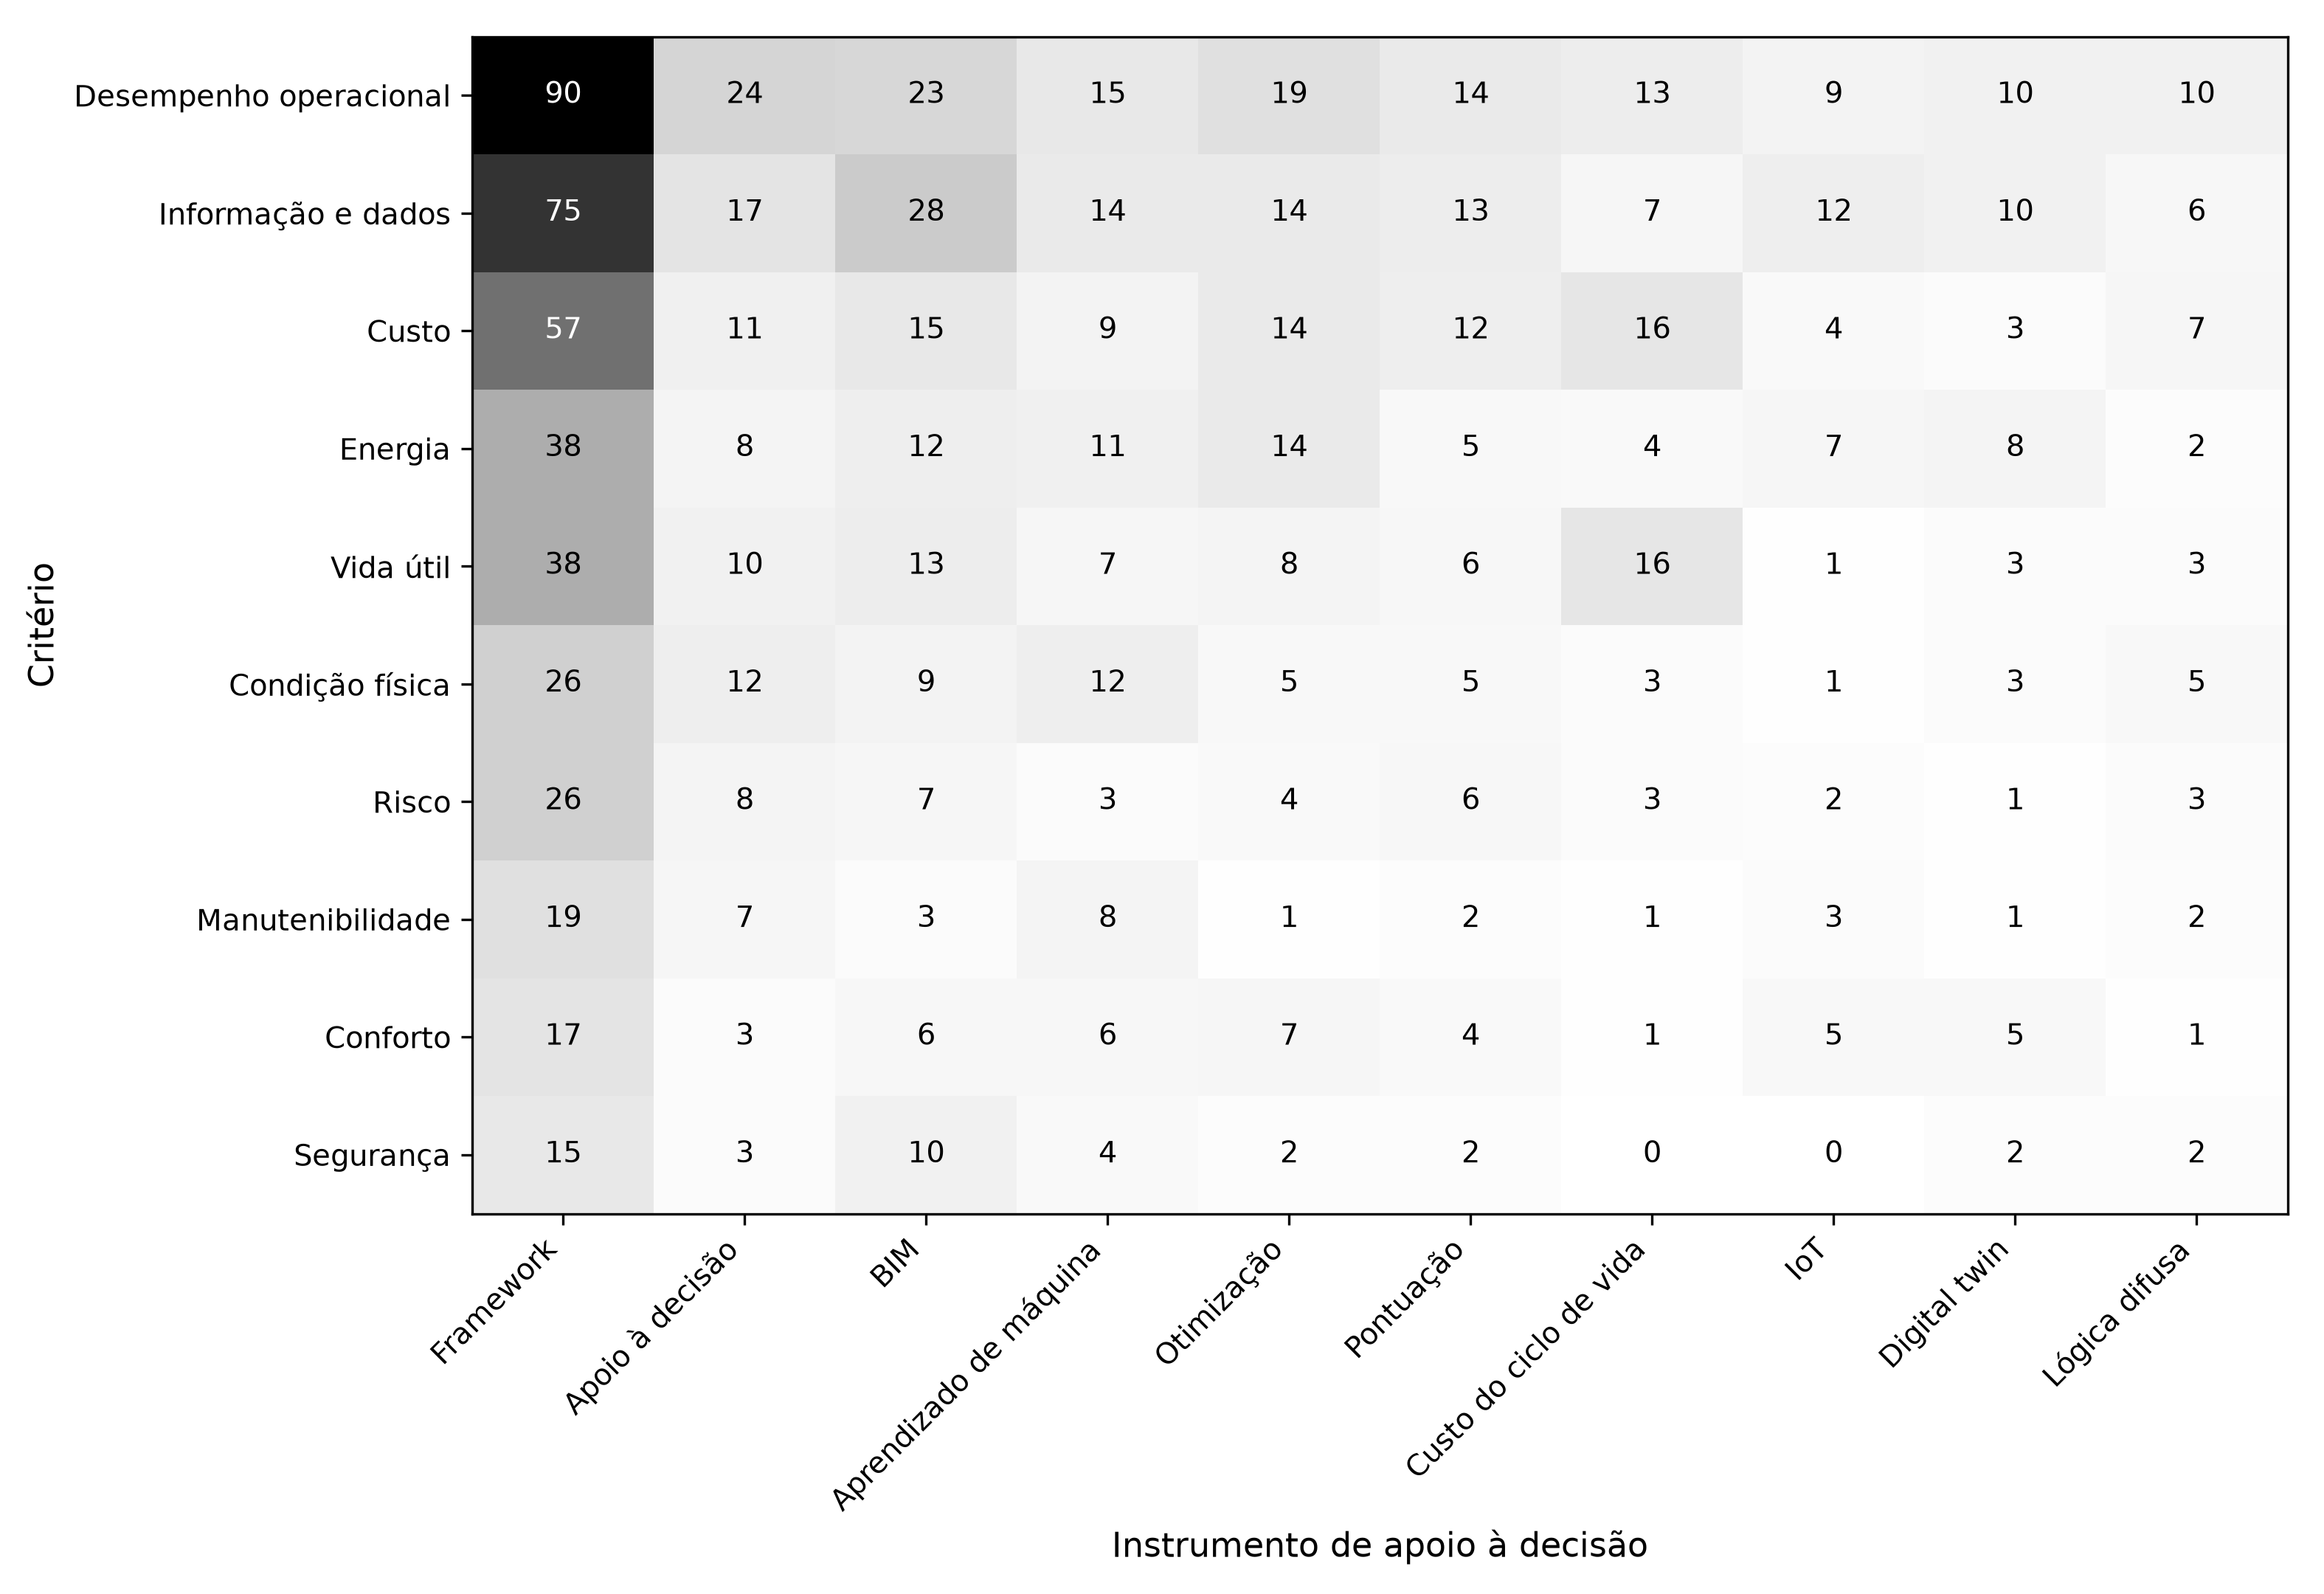
\includegraphics[width=0.98\linewidth]{figuras/figura13_heatmap_criterios_metodos_nucleo_ampliado_121.png}
\captiongrafico{Coocorrência entre critérios de priorização e instrumentos de apoio à decisão}
\label{fig:heatmap}
\end{figure}

O Gráfico~\ref{fig:matrizanalitica} reorganiza essas relações em cinco dimensões. A técnica-operacional apresenta 100 coocorrências com \texttt{framework}, 28 com \texttt{decision\_support} e 28 com BIM; em relação ao \texttt{framework}, a institucional apresenta 88 coocorrências, a ambiental 81, a econômica 56 e a social 54; identificada em 65 registros, a dimensão ciclo de vida atua transversalmente entre desempenho, custos e impactos no tempo.

\begin{figure}[htbp]
\centering
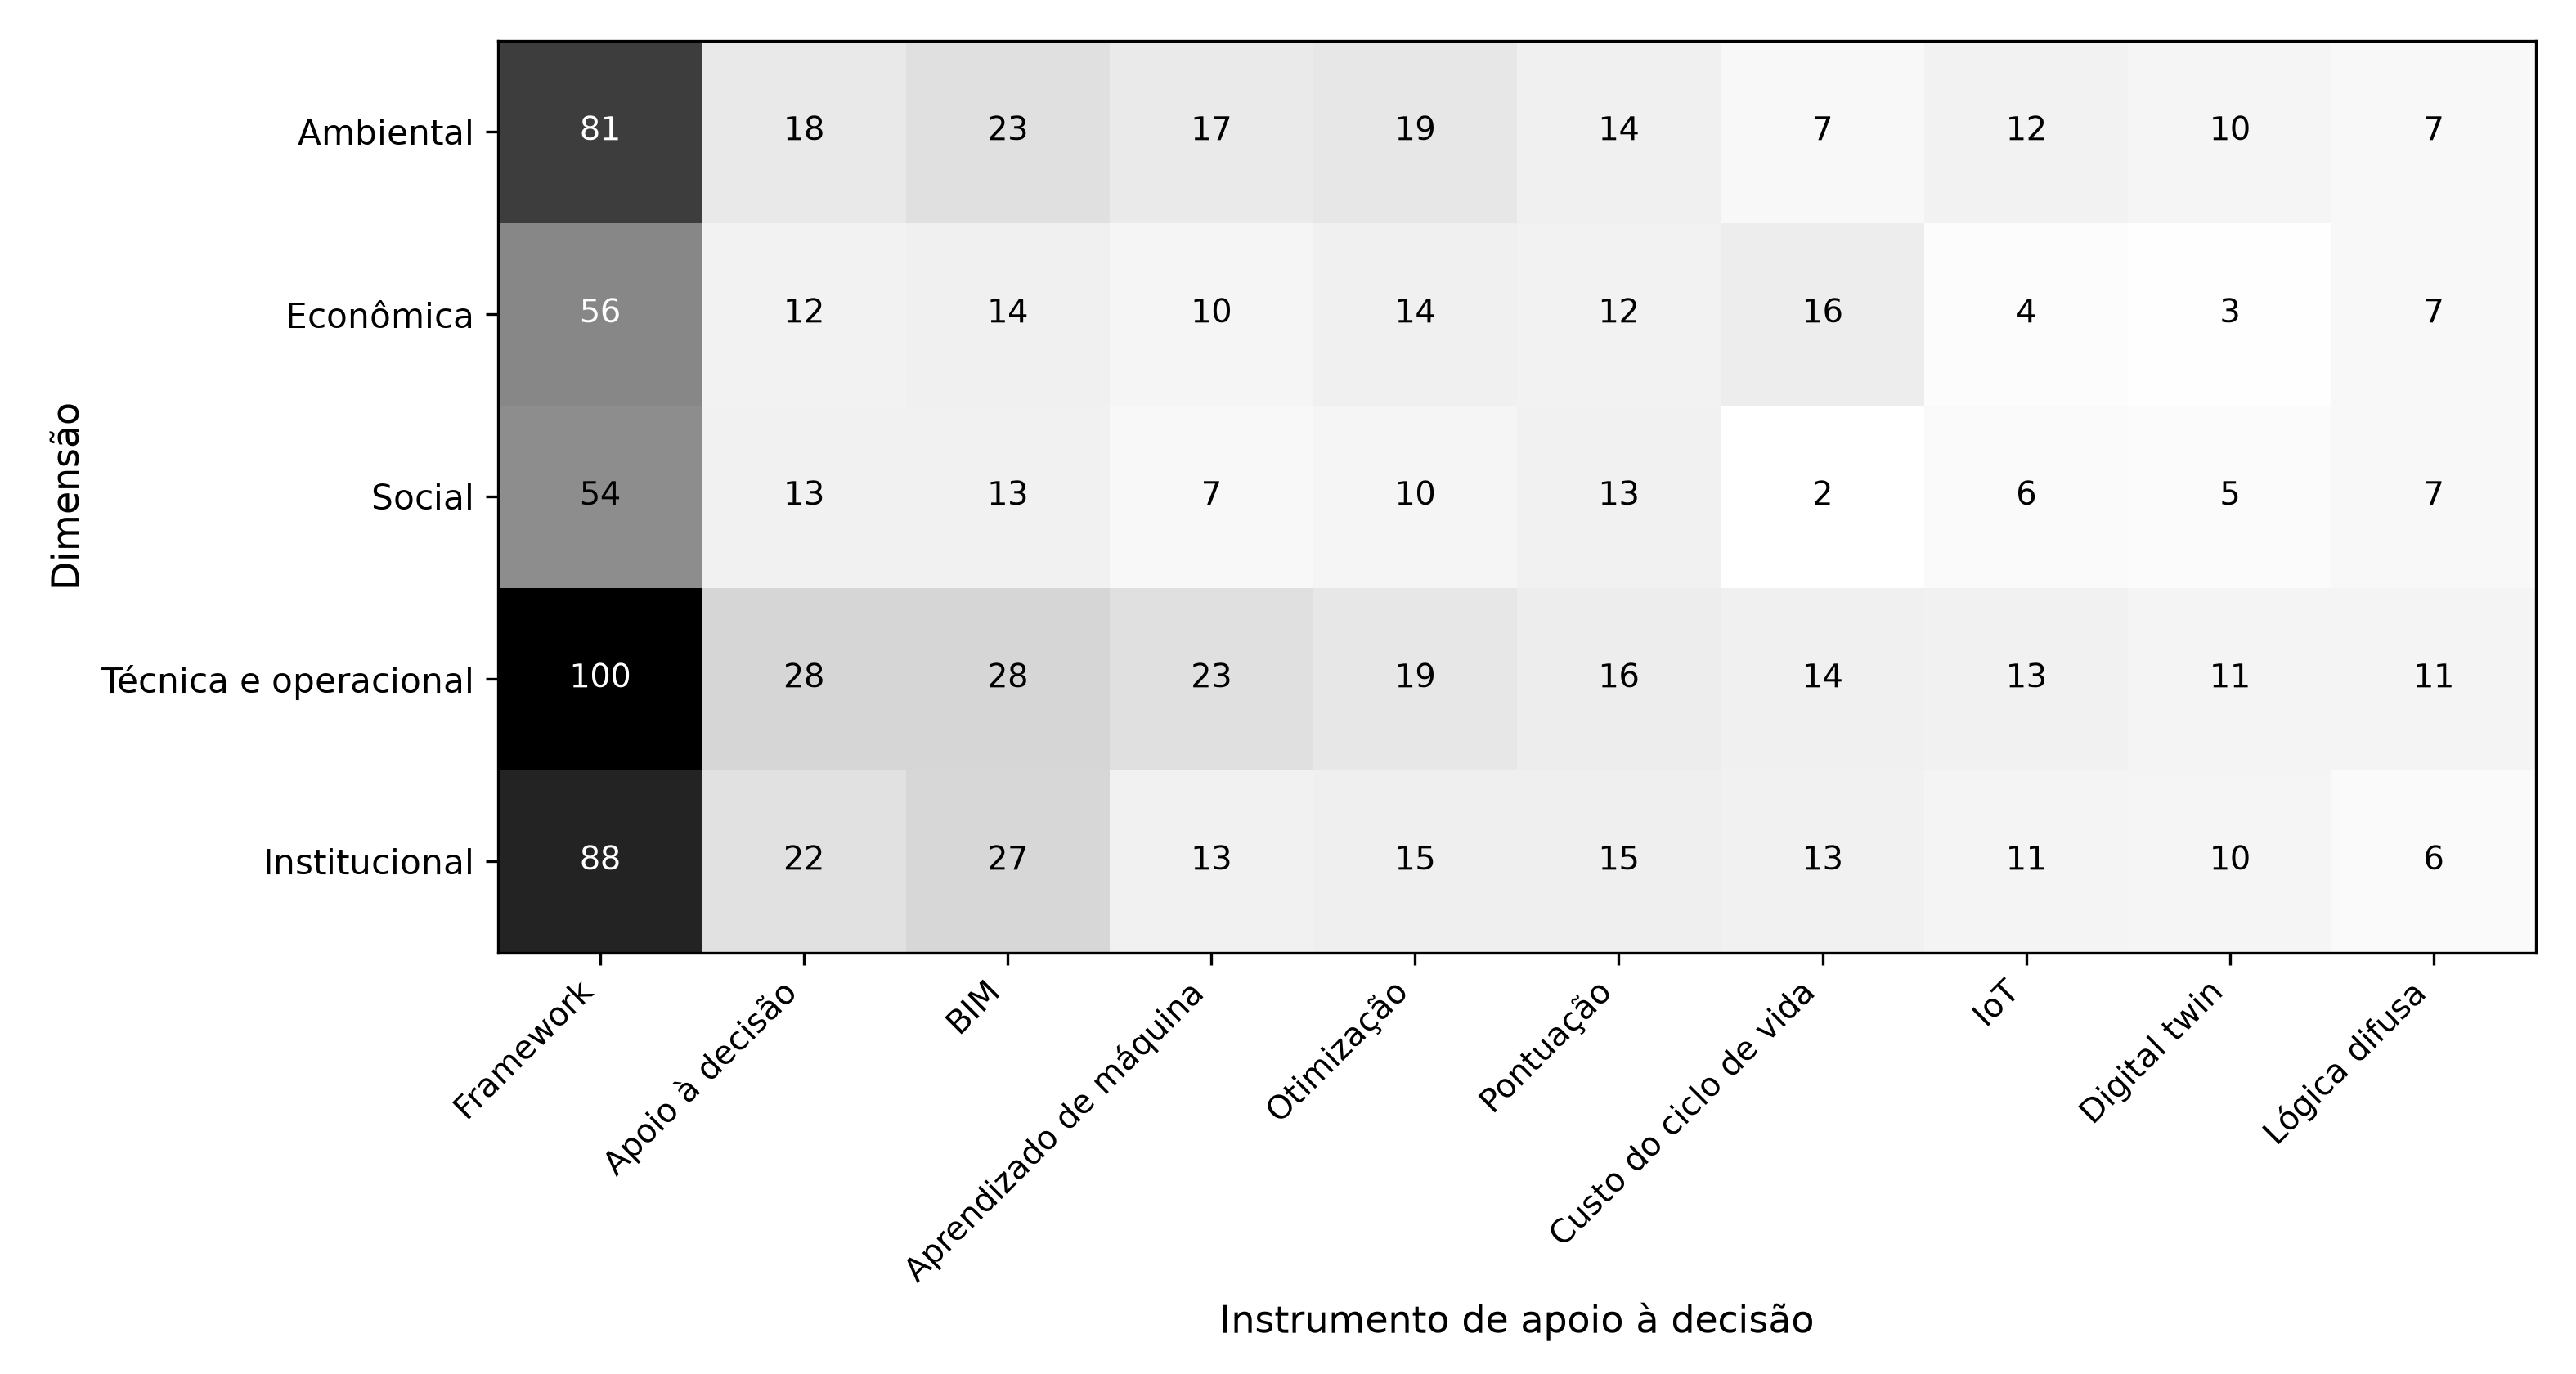
\includegraphics[width=0.98\linewidth]{figuras/figura14_matriz_analitica_dimensao_metodo_nucleo_ampliado_121.png}
\captiongrafico{Matriz de coocorrência entre dimensões de sustentabilidade e instrumentos de apoio à decisão}
\label{fig:matrizanalitica}
\end{figure}

A matriz que segue é uma síntese conceitual informada pela revisão, e não é um modelo validado nem um instrumento pronto para decisão; ela separa evidência extraída e especificação autoral. A dimensão ambiental reúne energia, emissões, água e resíduos, o custo constitui a dimensão econômica, segurança, conforto e satisfação integram a dimensão social, a técnica-operacional abrange desempenho, informação, vida útil, risco, condição, manutenibilidade e qualidade do serviço, e a institucional, presente em 97 registros, fundamenta os desdobramentos candidatos de conformidade, governança e capacidade de execução. As frequências sustentam a seleção inicial, enquanto pesos e importância normativa serão definidos na validação institucional. A Tabela~\ref{tab:protocolooperacional} liga critérios candidatos às evidências da revisão, e a Tabela~\ref{tab:especificacaoindicadores} apresenta, em plano separado, indicadores, fontes, periodicidades e direções propostos pelo autor para validação.

\begin{table}[htbp]
\centering
\caption{Rastreabilidade entre evidências e critérios candidatos}
\label{tab:protocolooperacional}
\scriptsize
\begin{tabularx}{\textwidth}{>{\RaggedRight\arraybackslash}p{2.4cm} >{\RaggedRight\arraybackslash}p{2.7cm} Y}
\toprule
Dimensão & Critério & Evidência da revisão \\
\midrule
Técnica-operacional & Desempenho e falha & Desempenho em 99 registros. A rede conecta gestão de facilidades a operação e manutenção. \\
Técnica-operacional & Informação e dados & Informação em 82 registros, BIM em 28 e \textit{digital twin} em 11. Perdas de informação foram observadas por \textcite{tan_fluxoinformacao_2018}. \\
Técnica-operacional & Condição e vida útil & Condição em 34 registros, vida útil em 44 e ciclo de vida em 65. A manutenibilidade é apoiada por \textcite{othman_manutenibilidadeesi_2023}. \\
Institucional & Conformidade & Dimensão institucional em 97 registros. \textcite{talib_hospitalfm_2013} aponta a necessidade de adaptação contextual. \\
Econômica & Custo & Custo em 63 registros. Previsão e ciclo de vida aparecem em \textcite{kim_estimativacustoseducacional_2018,nageli_ciclovida_2019}. \\
Ambiental & Energia & Dimensão ambiental em 92 registros e energia em 44. Ciclo de vida e carbono cresceram no período recente. \\
Social & Impacto nos usuários & Dimensão social em 59 registros, com conforto em 22, segurança em 18 e satisfação em nove. \\
\bottomrule
\end{tabularx}
\fonteautor
\end{table}

\begin{table}[htbp]
\centering
\caption{Proposição autoral de especificação operacional dos indicadores}
\label{tab:especificacaoindicadores}
\footnotesize
\begin{tabularx}{\textwidth}{>{\RaggedRight\arraybackslash}p{2.15cm} Y >{\RaggedRight\arraybackslash}p{2.3cm} >{\RaggedRight\arraybackslash}p{1.55cm} >{\RaggedRight\arraybackslash}p{1.7cm}}
\toprule
Critério & Indicador candidato & Fonte candidata & Apuração & Preferência \\
\midrule
Desempenho e falha & Ordens recorrentes por sistema, \% das ordens & Ordens de serviço & Mensal & Menor \\
Informação e dados & Ativos com cadastro e histórico completos, \% & Cadastro e ordens & Trimestral & Maior \\
Condição e vida útil & Índice de condição, escala institucional & Inspeção e cadastro & Semestral & Maior \\
Conformidade & Requisitos atendidos, \% & Laudos e auditorias & Anual & Maior \\
Custo & Custo estimado por área, R\$/m$^2$ & Orçamentos institucionais e base oficial aplicável & Semestral & Menor \\
Energia & Intensidade energética em base móvel de 12 meses, kWh/m$^2$ & Faturas ou medidores & Mensal & Menor \\
Impacto nos usuários & Reclamações por 100 usuários & Ouvidoria e chamados & Trimestral & Menor \\
\bottomrule
\end{tabularx}
\par\smallskip{\footnotesize Nota: indicadores, unidades, fontes, periodicidades e direções são proposições do autor para validação institucional. A revisão sustenta os critérios e a necessidade de rastreabilidade. Maior ou menor indica a direção desejável do indicador.\par}
\end{table}

A Figura~\ref{fig:fluxoprotocolo} resume o fluxo candidato, em que a unidade de comparação precede a coleta, e os critérios e indicadores são validados antes da elicitação dos pesos, com a divulgação da prioridade ocorrendo após a análise de sensibilidade e o registro das escolhas.

\begin{figure}[htbp]
\centering
\begin{tikzpicture}[
  node distance=7mm and 7mm,
  etapa/.style={draw, rounded corners, align=center, text width=3.6cm, minimum height=10mm, font=\scriptsize},
  veto/.style={draw, rounded corners, very thick, align=center, text width=11.7cm, minimum height=8mm, font=\scriptsize},
  seta/.style={-Latex, thick}
]
\node[etapa] (e1) {1. Definir unidade decisória};
\node[etapa, right=of e1] (e2) {2. Validar critérios e indicadores};
\node[etapa, right=of e2] (e3) {3. Verificar qualidade dos dados};
\node[etapa, below=of e3] (e4) {4. Parametrizar normalização, pesos e agregação};
\node[etapa, left=of e4] (e5) {5. Aplicar vetos e sensibilidade};
\node[etapa, left=of e5] (e6) {6. Registrar e publicar a prioridade};
\node[veto, below=of e5] (v) {Considera-se candidato a veto não compensatório qualquer risco estrutural, risco à vida, risco de incêndio ou descumprimento legal situado acima de limiar técnico ou normativo};
\draw[seta] (e1) -- (e2);
\draw[seta] (e2) -- (e3);
\draw[seta] (e3) -- (e4);
\draw[seta] (e4) -- (e5);
\draw[seta] (e5) -- (e6);
\draw[seta] (e5) -- (v);
\end{tikzpicture}
\caption{Fluxo candidato para validação e futura parametrização multicritério}
\label{fig:fluxoprotocolo}
\end{figure}

Na etapa 4, método, pesos e função de agregação serão definidos conforme o problema decisório, a participação institucional, a qualidade dos dados e o grau de compensação admissível. A análise de sensibilidade varia pesos, limiares e tratamento de ausências. Risco estrutural, risco à vida, incêndio e descumprimento legal formam vetos candidatos, com limiares estabelecidos por norma, laudo ou autoridade competente \parencite{abnt_nbr5674_2012,araujoneto_manutencaolegislacao_2015}; o ciclo de vida permanece transversal para evitar dupla contagem.

A especificação proposta liga, assim, os critérios sustentados pela revisão a indicadores candidatos e a um fluxo de validação, convertendo dimensões e critérios recorrentes em etapas verificáveis e respondendo à RQ0. A baixa presença lexical de ODS e ESG, diante da recorrência de energia, emissões, segurança, conforto e governança, indica aproximação substantiva ainda pouco expressa por esses rótulos \parencite{ramantswana_esgfm_2026}. As coocorrências descrevem associações documentais, e a avaliação institucional determinará importância, pesos, método e robustez segundo a força e a disponibilidade dos dados, completando a cadeia entre evidência científica, dimensão, critério, indicador observável, parametrização multicritério futura, veto não compensatório e decisão pública rastreável.
